\documentclass{beamer}

\usepackage[frenchb]{babel}
\usepackage[T1]{fontenc}
\usepackage[latin1]{inputenc}
\usepackage{tikz}
\usetikzlibrary{quotes,angles,calc,intersections,babel,through,backgrounds,angles,positioning}
\usepackage{rotating}

\usetheme{Warsaw}

\title{Soutenance bibliographique}
\author{BESSENG A IREH Guy Raymond}
\institute[]{Universit� Paul Sabatier}
\setbeamertemplate{caption}{\raggedright\insertcaption\par}
\begin{document}

\maketitle
\section{introduction}
\begin{frame}
\frametitle{Article}
\begin{center}
Shape and motion of drops sliding down an inclined plane

By NOLWENN LE GRAND, ADRIAN DAERR AND LAURENT LIMAT

\end{center}
\end{frame}

\begin{frame}
\frametitle{Dispositifs exp�rimentales}
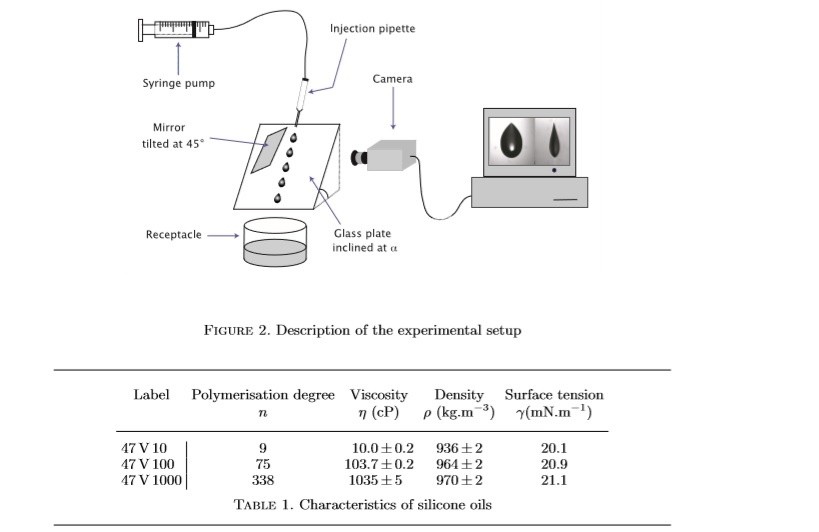
\includegraphics[scale = 0.5]{Experiment.jpg}
\end{frame}


\begin{frame}
\frametitle{Observations}
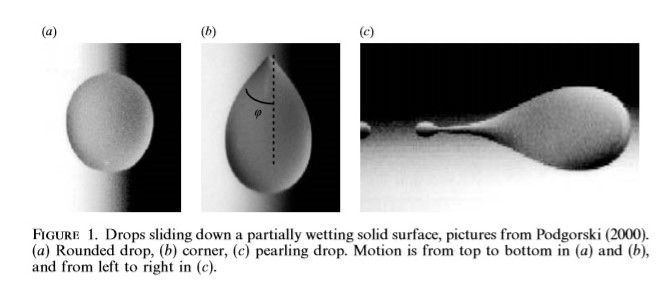
\includegraphics[scale = 0.5]{goutte1.jpg}
\end{frame}


\begin{frame}
\frametitle{Transtion d'une forme � l'autre}
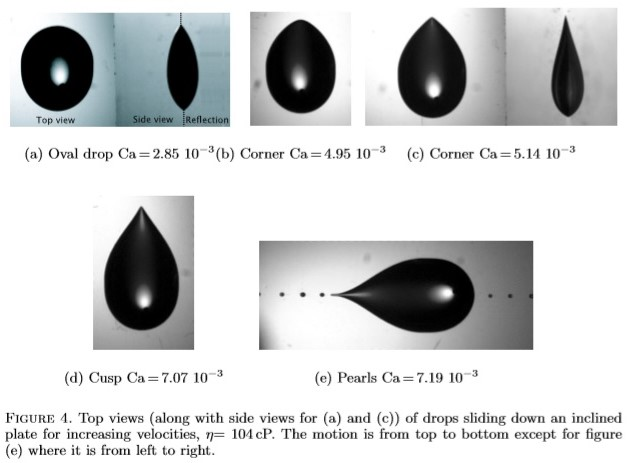
\includegraphics[scale = 0.5]{ovale_pointue.jpg}
\end{frame}


\begin{frame}
\frametitle{Notations}
\begin{itemize}
	\item angle statique $\theta_{s} = \frac{\gamma_{sl}-\gamma_{sg}}{\gamma}$
	\item Le nombre capillaire $C_{a} = \frac{\text{effets visqueux}}{\text{effets inertiel}} = \frac{\eta U}{\gamma}$
	\item $B_{O} = \frac{\text{effets gravitaires}}{\text{effets inertiels}} = B_{O}\sin\alpha = V ^ {2/3} (\rho g / \gamma)$
	\item $B_{O_{\alpha}} = B_{O}\sin\alpha = V ^ {2/3} (\rho g  / \gamma)\sin \alpha$
\end{itemize}
\end{frame}

\begin{frame}
\frametitle{Bilan des forces}
\begin{center}
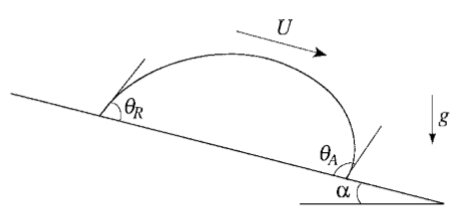
\includegraphics[scale = 0.2]{Bilan.png}
\end{center}
\begin{itemize}
	\item Le poids : $\rho g V \sin \alpha$
	\item la force de frottement: $\eta U V^{1/3}$
	\item la tension de surface : $\gamma \Delta \theta = \gamma \omega \left( \cos (\theta_{R} - \theta{A} ) \right)$ 
\end{itemize}
\end{frame}


\begin{frame}
\frametitle{Comparaisons avec des mod�les}
\begin{itemize}
	\item De Gennes : $ \theta \left(\theta^{2} - \theta_{s}^{2}\right) = \pm 6\ln\left(\frac{b}{a}\right)C_{a}$
	\item Cox et Voinov : $\theta^{3} - \theta_{s}^{3} = \pm 9\ln\left(\frac{b}{a}\right) C_{a}$
	\item Cin�tique mol�culaire: $\left(\theta^{2} - \theta_{s}^{2}\right) = \frac{\nu NkT}{2\pi fL_{m}h}C_{a}$
        \item Lin�aire : $\theta - \theta_{s} \propto \pm U$
\end{itemize}

\end{frame}

\begin{frame}
\begin{figure}
\centering
\begin{tikzpicture}[scale=1.5]
\node[below] (O) at (0,0) {$O$};
\node[above] (C) at (155:0.5) {$\gamma_{lg} = \gamma$};
\node[below] (A) at (-0.8,0) {$\gamma_{sl}$};
\node[below] (B) at (0.6,0) {$\gamma_{sg}$};
\draw (-5,0) -- (2,0);
\filldraw[fill = blue] (0,0) arc (70:110:5) -- cycle;
\draw[->,color = red,rotate = 160] (0,0) -- (0.7,0);
\draw[->,color = red] (0,0) -- (0.5,0);
\draw[<-,color = red] (-0.7,0) -- (0,0);
pic [draw=red, angle radius=0.2,
	"$\alpha$"] {angle = (0.0,0)--(-0.7,0)--(160:0.7)};
\end{tikzpicture}
\caption{Mouillage partiel : $ \gamma_{sg}-\gamma -\gamma_{sl}  = s < 0$}
\end{figure}

\end{frame}


\begin{frame}
\frametitle{Approximation de lubrification}
\begin{itemize}
\item \[\frac{ \partial \vec{v} }{ \partial t } + \left(\vec{v} \cdot \overrightarrow{\mathrm{grad}}\right)\vec{v} = - \frac{1}{\rho}\,\overrightarrow{\mathrm{grad}}\,p + \nu \Delta\,\vec{v}\]
\end{itemize}

\end{frame}




\begin{frame}
  \frametitle{Conclusion}
\end{frame}

\begin{frame}
\frametitle{Questions}
  \center{Avez-vous des questions ?}
\end{frame}



\end{document}
